\documentclass[11pt]{article}
\usepackage{common}
\usepackage[usenames, dvipsnames]{color}
\usepackage{setspace}
\usepackage{booktabs}
\usepackage{multirow}
\usepackage{framed}

\title{CS207 Algorithm Analysis: Kernel Density Estimation}
\author{Gioia Domined\`o \and Nicolas Drizard \and Kendrick Lo \and Malcolm Mason Rodriguez}

\begin{document}
\maketitle{}

\pagestyle{plain}
\pagenumbering{arabic}

\section{Introduction}

Kernel Density Estimation (KDE) is a non-parametrical statistical technique that is used to estimate the probability density function (PDF) of a random variable based on a finite data sample\footnote{https://en.wikipedia.org/wiki/Kernel\_density\_estimation}.  Mathematically, we can denote the KDE of the PDF of independent and identically distributed (\textit{iid}) random variables $X=\{x_1, x_2, ..., x_n\}$ as:

\begin{equation} \label{eq:kde}
\hat{f}_h(x) = \frac{1}{n} \sum_{i=1}^n K_h(x - x_i) = \frac{1}{nh} \sum_{i=1}^n K \Big( \frac{x - x_i}{h} \Big)
\end{equation}

\noindent where $K(\cdot)$ represents the \textit{kernel} and $h$ represents the \textit{bandwidth} (i.e. a smoothing parameter). We note that $\hat{f}_h(x)$ denotes the estimated PDF at a particular point $x$, and that the entire data set $X$ is used to calculate it. \medskip

\noindent Various kernels are used in practice (e.g. Gaussian, Epanechnikov, exponential, etc.), all of which meet the criteria of being non-negative functions with mean zero that integrate to one. Similarly, different (strictly positive) values of $h$ can be chosen depending on the data set in question. Figure \ref{fig:kde_params} illustrates how the choice of these two parameters affects the shape of the estimated PDF.

\begin{figure}[h!]
\centering
\subfloat[Changing the kernel (bandwidth$=0.2$)]{\label{fig:kde_params_k}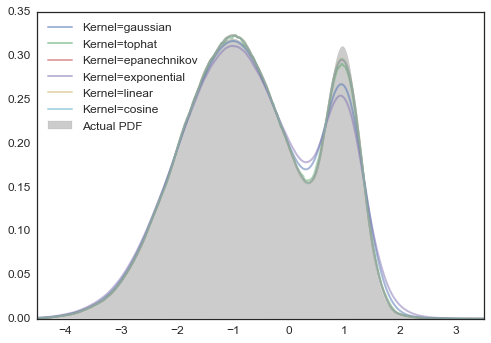
\includegraphics[width=3in]{img/change_k}}
\subfloat[Changing the bandwidth (gaussian kernel)]{\label{fig:kde_params_bw}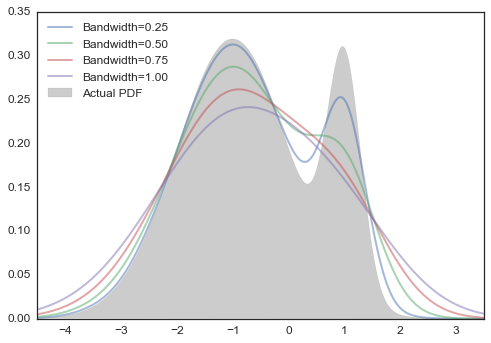
\includegraphics[width=3in]{img/change_bw}}
\caption{Impact of KDE parameters}
\label{fig:kde_params}
\end{figure}

\newpage

\section{Algorithm}

A discussion on the ``best" parameters for KDE is beyond the scope of this paper.  For ease of comparability, all our experiments are based on a Gaussian kernel and a bandwidth of $0.2$. Figure \ref{fig:sample_kde} shows the result of running the Scikit Learn KDE algorithm with these parameters on 100K one-dimensional random variables drawn from a bimodal distribution, where the PDF is plotted at 1K evenly-spaced values of $x$.

\begin{figure}[h!]
\centering
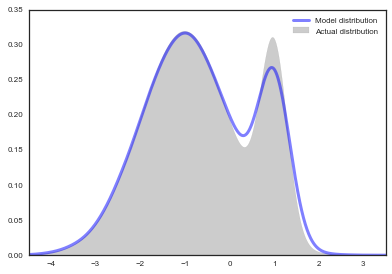
\includegraphics[width=4in]{img/sample_kde.png}
\caption{Sample KDE output}
\label{fig:sample_kde}
\end{figure}

\noindent We started by implementing a ``pure" Python version of KDE; in keeping with that objective, we only used lists. We can see from the code below that the KDE algorithm is a direct application of Equation \ref{eq:kde}. The double loop, which is necessary due to the use of lists, immediately stands out as a significant source of inefficiencies.

\begin{framed}
\begin{singlespacing}
\begin{scriptsize}
\begin{verbatim}
def gaussian(x):
    '''
    Returns the Gaussian function for a given input variable.
    
    Parameters
    ----------
    x : float
        the x-value at which to evaluate the Gaussian function
        
    Returns
    ----------
    gaussian : float
        the result of evaluating the Gaussian function at x
    '''
    return np.exp(-1.0 * (x**2) / 2) * (1.0 / np.sqrt(2.0 * np.pi))
\end{verbatim}
\end{scriptsize}
\end{singlespacing}
\end{framed}

\newpage

\begin{framed}
\begin{singlespacing}
\begin{scriptsize}
\begin{verbatim}
def naive_kde(x, x_grid, h):
    '''
    Calcalates the KDE PDF estimate, based on a Gaussian kernel.
    
    Parameters
    ----------
    x : list
        iid random variables that are used to calculate the KDE estimate
    x_grid : list
        values along which to calculate the KDE estimate
    h : float
        bandwidth parameter for the KDE estimate
        
    Returns
    ----------
    estimates: list
        KDE estimates for all values of x_grid
    '''
    global N # number of iid random variables
    estimates = [0] * len(x_grid)
    
    for j, gridpt in enumerate(x_grid):
        for i in range(N):
            val_in_sum = gaussian((x[i] - gridpt) / h)
            estimates[j] += val_in_sum
        
        estimates[j] = estimates[j] / (N * h)
    
    return estimates
\end{verbatim}
\end{scriptsize}
\end{singlespacing}
\end{framed}

\noindent Before moving on to the Scikit Learn implementation, we tested the effect of switching from lists to Numpy arrays and vectorizing the inner loop. This simple change, which is shown in the code below, reduced the runtime from nearly 300 seconds to just over 1 second!

\begin{framed}
\begin{singlespacing}
\begin{scriptsize}
\begin{verbatim}
def vectorized_kde(x, x_grid, h):
    '''
    Calcalates the KDE PDF estimate, based on a Gaussian kernel.
    Inputs
    ----------
    x      : An array of iid random variables that are used to calculate the KDE estimate
    x_grid : An array of values along which to calculate the KDE estimate
    h      : Float, the bandwidth parameter for the KDE estimate
    Returns
    ----------
    An array of KDE estimates for all values of x_grid.
    '''    
    global N # number of iid random variables

    estimates = np.zeros(len(x_grid))
    
    for j, gridpt in enumerate(x_grid):
        val_in_sum = gaussian((x - gridpt)/h)  # returns vector of dim N
        estimates[j] = np.sum(val_in_sum) / (N * h)
    
    return estimates
\end{verbatim}
\end{scriptsize}
\end{singlespacing}
\end{framed}

\newpage

\section{Scikit Learn Optimizations}

After completing our Python implementation, we next moved on to examine the Scikit Learn implementation\footnote{The full source code is available at https://github.com/scikit-learn/scikit-learn/tree/master/sklearn/neighbors.} and analyze its optimizations.

%default distance metric = euclidean distance

%FFT-based computation
%For large datasets, a kernel density estimate can be computed efficiently via the convolution theorem using a fast Fourier transform. This requires binning the data, so the approach quickly becomes inefficient in higher dimensions. Of the four algorithms discussed here, only Statsmodels' KDEUnivariate implements an FFT-based KDE. As we'll see below, the FFT provides some computational gains for large numbers of points, but in most situations is not as effective as tree-based KDE implementations.


%requires homogenous datasets (vs Statsmodels' KDEMultivariate - can handle mix of  mix of continuous, ordered discrete, and unordered discrete variables)

%about a dozen distance metrics??

\begin{table}[h!]
\centering
\begin{tabular}{@{}ll@{}}
\toprule
Implementation			& Runtime (seconds)       	\\
\midrule
Naive Python			& 298.28				\\
Vectorized Python		& 1.34				\\
Scikit Learn			& 5.73				\\
\bottomrule
\end{tabular}
\caption{Comparing one-dimensional KDE implementations}
\label{compare_kde}
\end{table}


%\section{Additional Considerations}
%KDE estimation in higher-dimensional space?

\end{document}
